\chapter{Metodología}
\section{Levantamiento de información}
El departamento de ingeniería mecánica en el Campus Casa Central, posee una máquina de fatiga (MF) uniaxial en flexión en el laboratorio de tecnología mecánica que se encuentra en la universidad hace más de 50 años, sin saber su fecha exacta de adquisición. La medición de fatiga es realizada a través del método de \textit{esfuerzo-vida}, utilizando la configuración de \textit{rotating bending}, ambos descritos en el capítulo anterior. La información existente sobre la máquina de ensayos es escasa, principalmente por su antigüedad, la perdida de documentos y obsolescencia de la electrónica. Por lo mismo, parte del trabajo de esta memoria se centra en lograr rescatar información y su posterior comprensión para lograr tener operativa la máquina de fatiga.

\begin{figure}[h]
\centering
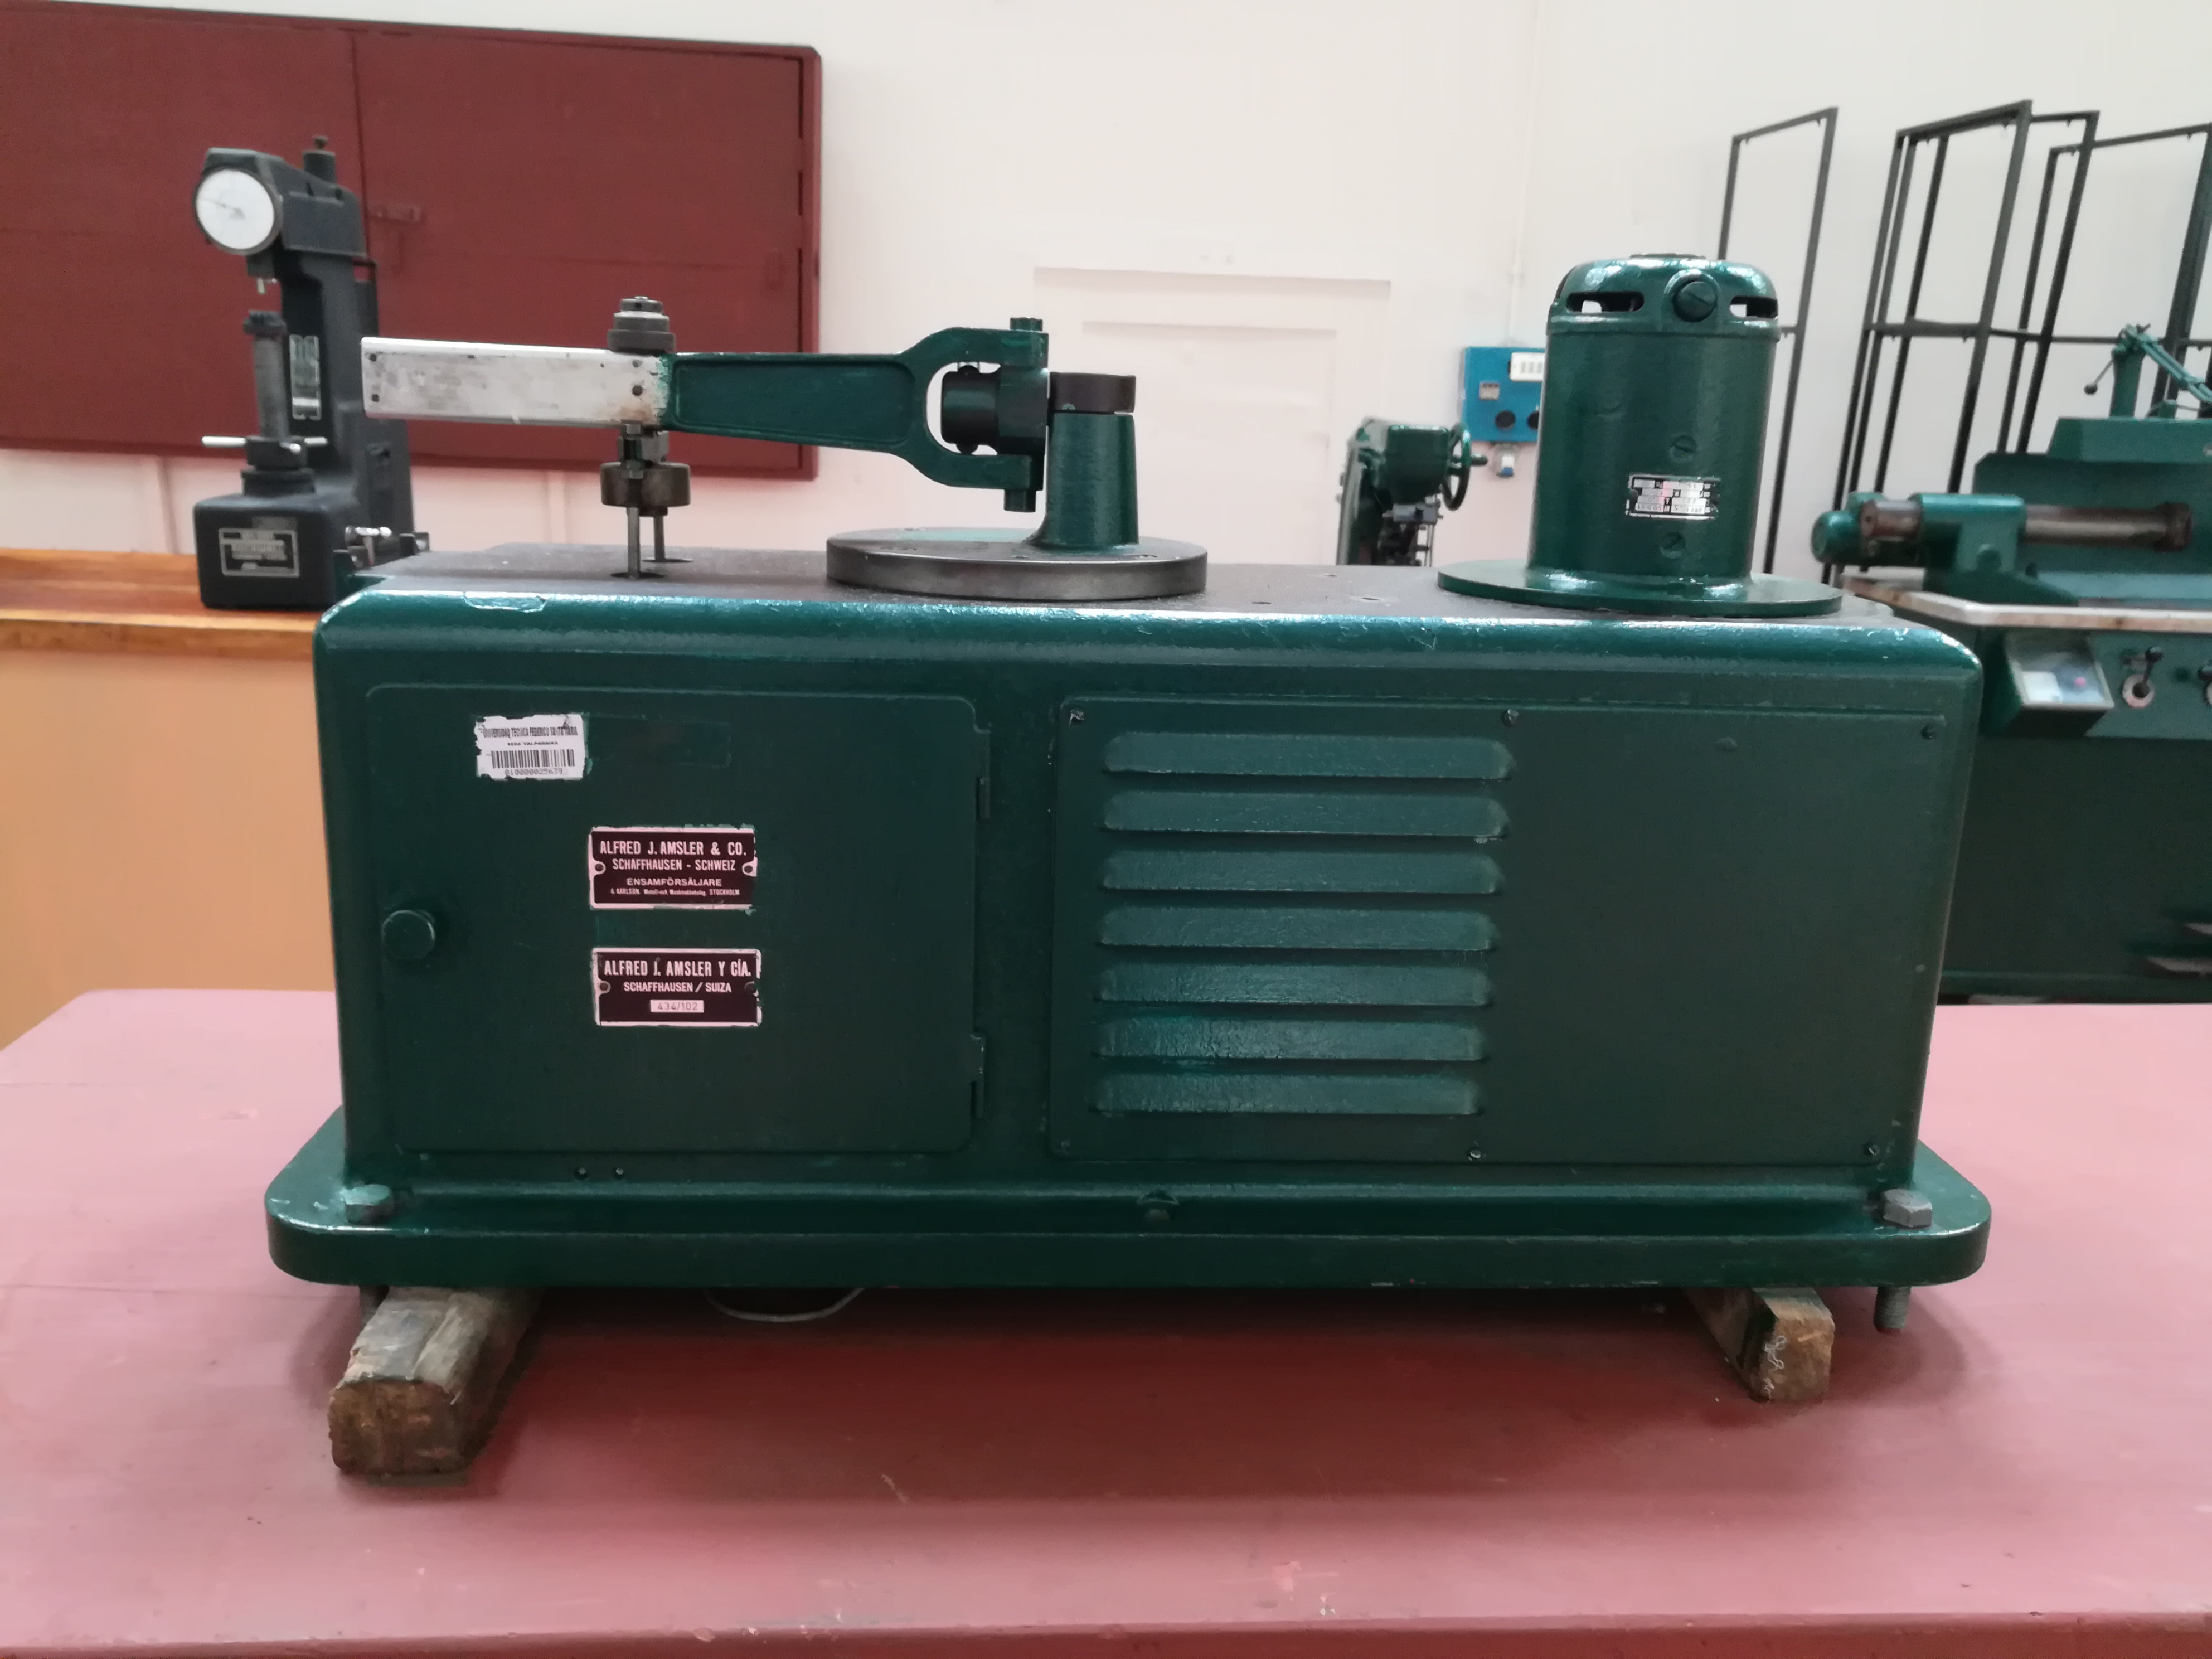
\includegraphics[scale=0.05]{Imagenes/maq_del.jpg}
\label{fig:maq_del}
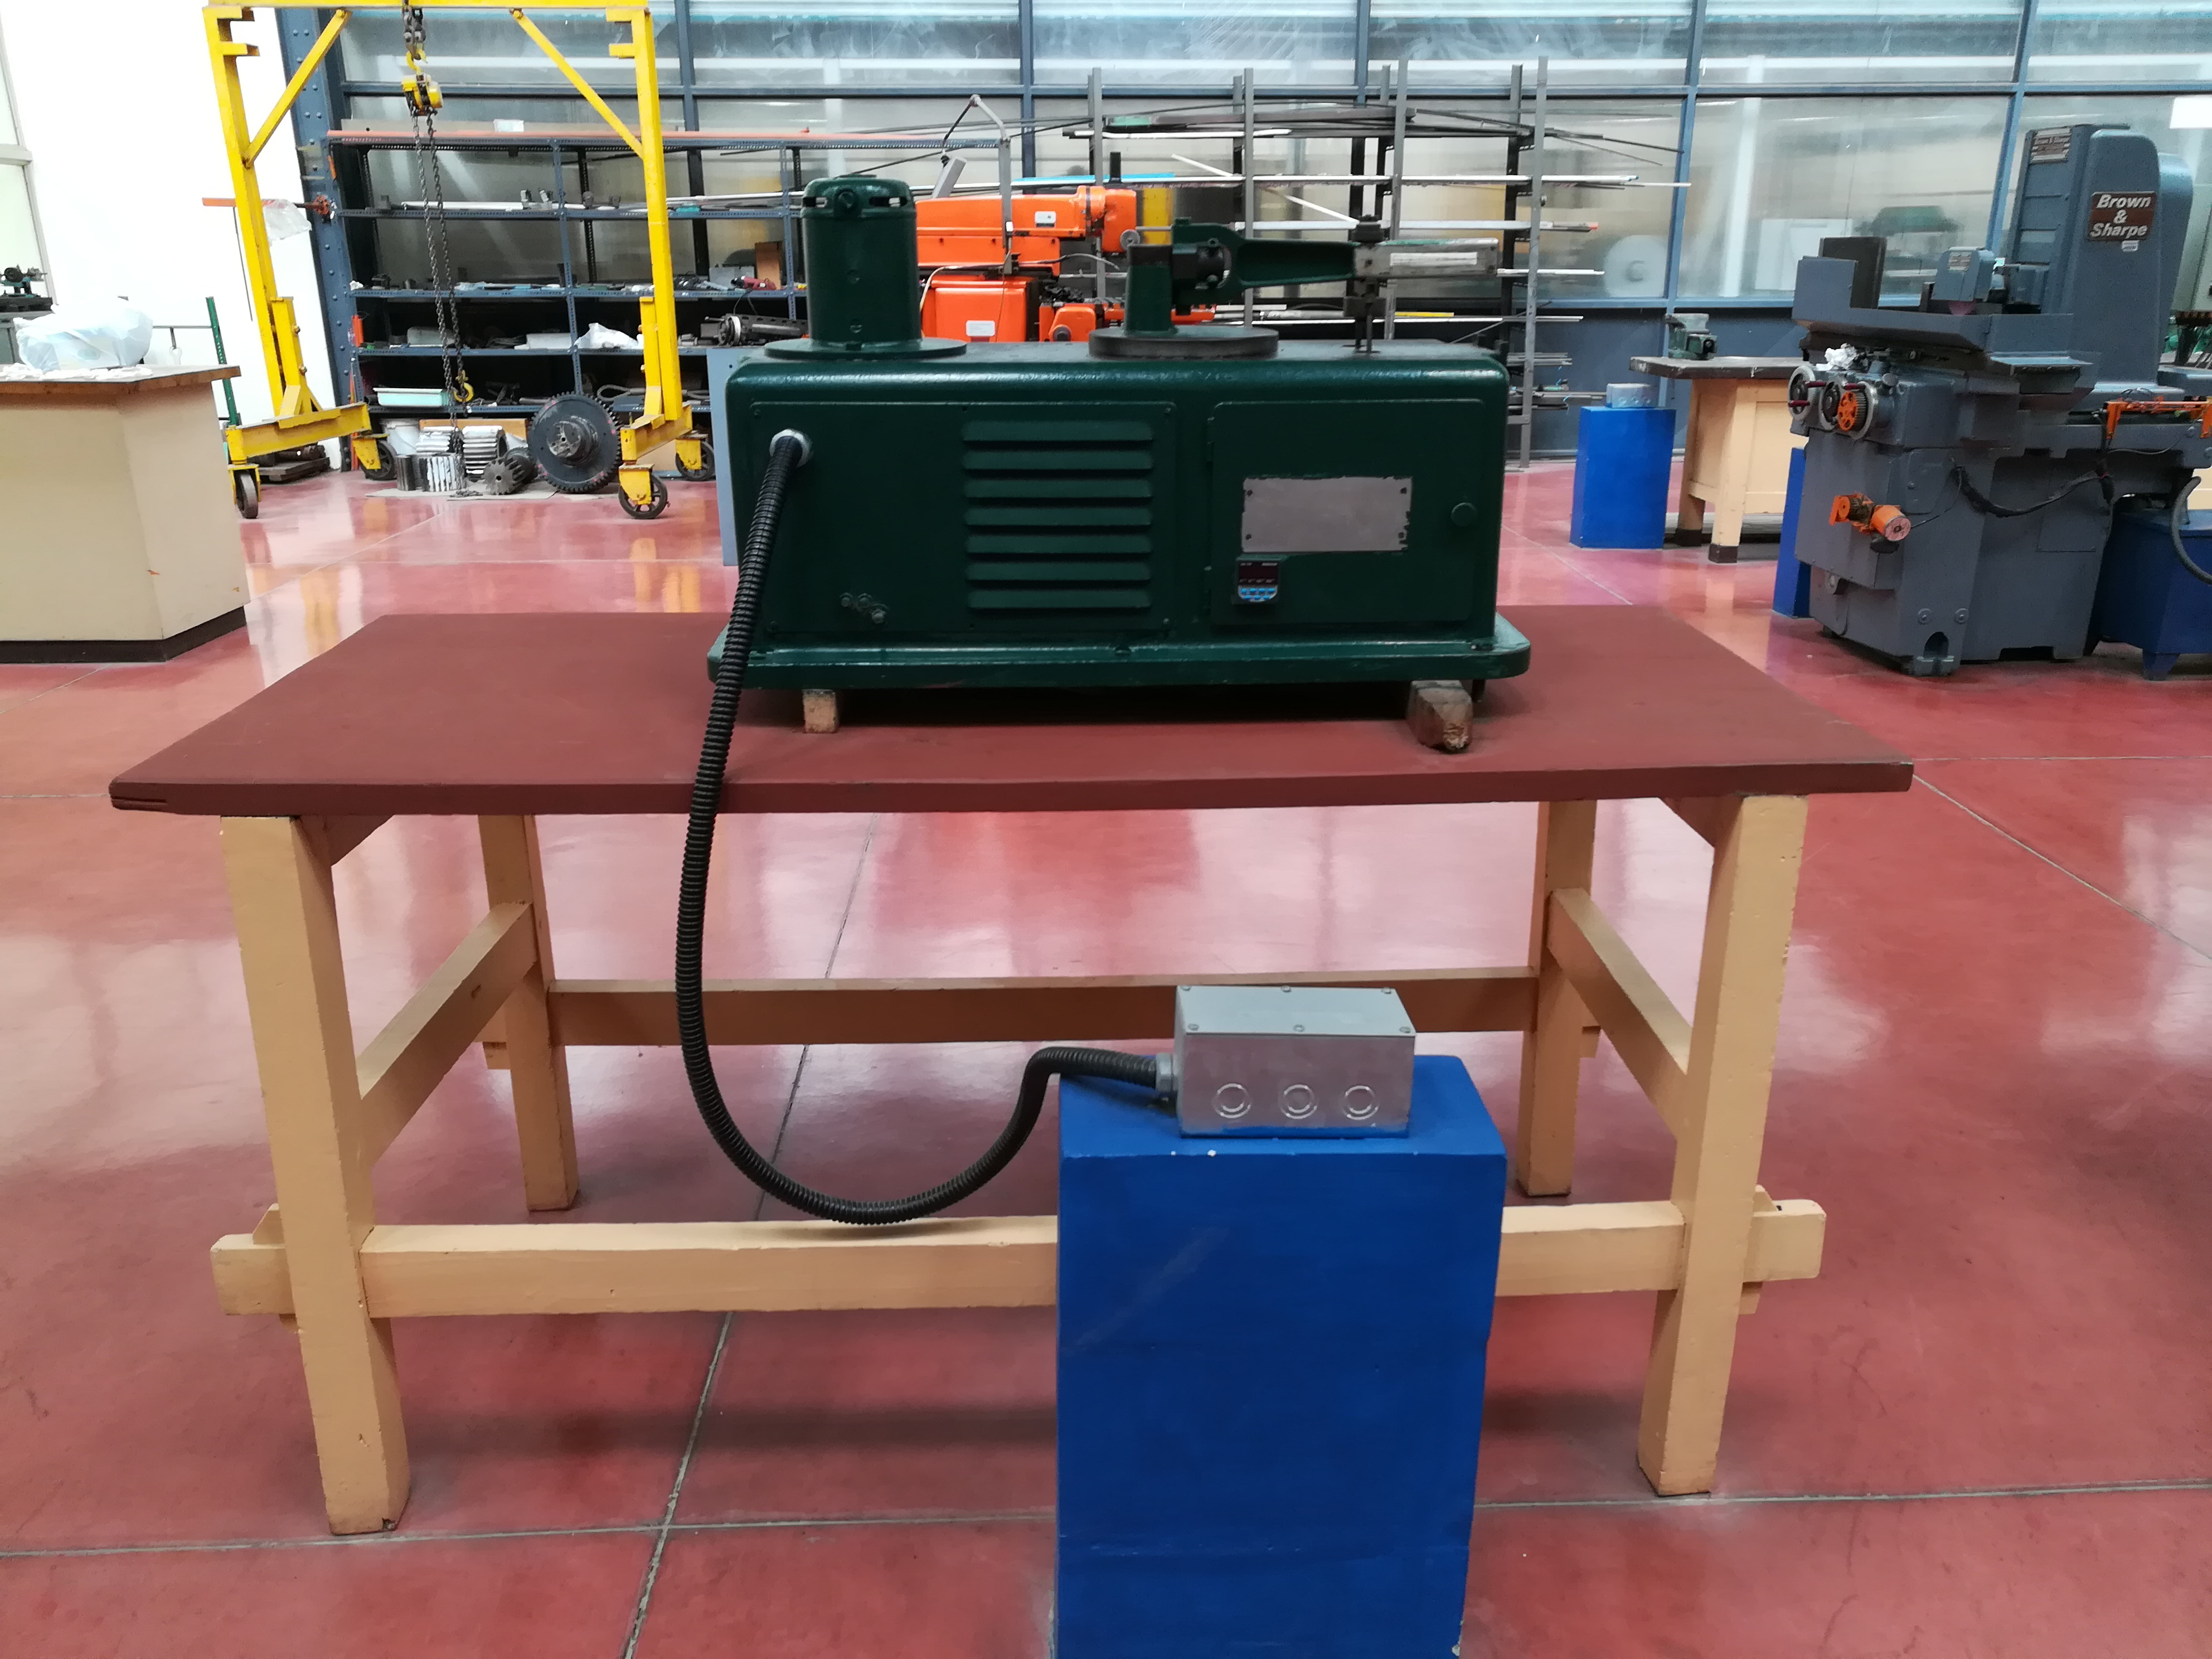
\includegraphics[scale=0.05]{Imagenes/maqfull_post.jpg}
\label{fig:maqfull_post}
\caption{Máquina de fatiga en flexión en el laboratorio de tecnología mecánica}
\label{fig:maq_fat}
\end{figure}

\subsection{Estado actual y antecedentes}
Actualmente la máquina no puede ser utilizada por no estar anclada, estando apoyada sobre dos listones de madera, que a su vez, están sobre una mesa de madera como se aprecia en la figura REF. Por consiguiente, la máquina al ser utilizada comienza a vibrar, saltar y desplazarse lateralmente, lo que impide su uso prolongado por motivos de seguridad. Es decir, no es posible realizar correctamente un ensayo de fatiga de ningún material ni configuración.

A partir de información verbal entregada por el profesor Fernando Rojas, se cree que la máquina fue adquirida por el departamento hace, al menos, 50 años atrás. Fue fabricada en Suiza por \textit{Alfred J. Amsler \& Co.} y su estructura completa es de acero fundido. Previo a la modificación actual del laboratorio, la máquina se encontraba anclada al piso con un bloque de concreto que fue demolido durante la remodelación, momento desde el cual se encuentra sin una solución definitiva. Más aún, varios equipos y máquinas de ensayo del laboratorio no se encuentran ancladas al piso ni con una instalación definitiva impidiendo su uso.

La única modificación que posee la máquina, según la información recopilada, consiste en el cambio del contador de revoluciones o ciclos realizados en un ensayo de fatiga. Esta actualización consistió en sacar el contador mecánico original y reemplazarlo por un contador electrónico, el cual tiene sus controles y el display adosada a su estructura, como se puede apreciar en la figura \textcolor{red}{agregar imagen del contador}. 

El sistema eléctrico de la máquina permanece intacto, la cual se encuentra conectada a la red de la universidad. Conserva su motor eléctrico original junto a un conjunto eléctrico cuya función es suministrar energía de manera continua y estable al motor, para evitar que el ensayo de fatiga se pueda ver afectado por problemas y las variaciones del suministro eléctrico. El motor es de \textcolor{red}{corriente continua} con velocidad constante y sus especificaciones se pueden ver en la tabla \ref{tab:motor_maq}:

\begin{table}[h]
\centering
\begin{tabular}{ll}
\hline
Especificaciones Motor                            & Valor   				\\ \hline
Tensión                                           & 220 {[}V{]}        		\\
Corriente                                         & 0,8 {[}A{]}        		\\
Factor de potencia ($\cos \varphi$)				  & Sin información    		\\
Potencia                                          & 100 {[}W{]}        		\\
Velocidad                                         & 1500 {[}rev/min{]} 		\\ \hline
\end{tabular}
\caption{Especificaciones del motor de la máquina de fatiga.}
\label{tab:motor_maq}
\end{table}

Otro elemento distinto al original consiste en la correa de transmisión entre el motor eléctrico y el disco desbalanceado. La original consistía en una correa de cuero plana y cruzada, sin información respecto a su empalme. La correa actual consiste también en una correa plana y cruzada, sin embargo, su material es tela y el empalme es realizado a mano con hilo acerado. Cabe destacar que lo poco usual de las dimensiones, características y la necesidad de hacer el empalme en la misma máquina, dificulta la búsqueda de una correa que pueda cumplir de manera óptima la transmisión de potencia. Parte de estas dificultades se deben a que el sistema de transmisión no ha sido modificado donde sus poleas tienen dimensiones, tanto de diámetro como de ancho, que no están normalizadas o se encuentran fuera de catálogo de mucho proveedores. 

Por otro lado, los elementos de agarre de la probeta no tienen modificaciones conocidas, tanto el brazo que recibe el movimiento como el agarre empotrado a la estructura de la máquina. La fabricación de las probetas utilizadas se realiza en el mismo laboratorio a partir de acero AISI 1020 o 1040, el cual para conseguir las dimensiones de la figura REF. se debe cortar y tornear.

Finalmente, para realizar los ensayos en distintas configuraciones existen distintas masas (figura REF) que desequilibran el disco rotativo, como se verá en la sección \ref{sec:funcionamiento}, y estas combinaciones se especifican en una tabla de cargas (Anexo REF). Sin embargo, se desconoce el origen, y en consecuencia, la fiabilidad de la información contenida en esta tabla.

\subsection{Funcionamiento}
\label{sec:funcionamiento}
La máquina de fatiga tiene como objetivo lograr que para cada ciclo se ejerza el mismo esfuerzo determinado sobre la probeta, en forma de flexión. Para lograr esto, el mecanismo utilizado es un disco desequilibrado girando a una velocidad constante $\dot{\theta}$, la fuerza es transmitida hasta un brazo que sostiene a su vez a la probeta, generando flexión en la probeta con un doble empotramiento. La velocidad $\dot{\theta}$ del disco se transmitida desde el motor eléctrico a través de poleas y una correa de transmisión en una relación de 1:1 \textcolor{red}{revisar}, a una velocidad de 1500 revoluciones por minuto. Así, para realizar las mediciones de fatiga a distintas cargas se modifica el desequilibrio del disco a través de un conjunto de masas, mostradas en la figura REF, que permiten generar distintas configuraciones y, por consiguiente, esfuerzos en la probeta.

\textcolor{red}{Agregar imagen de contrapesos}

Los elementos utilizados para desbalancear son 6 discos pequeños de X \textcolor{red}{medir radio masas} a Y de diámetro. Estos son enumerados del 1 al 5, donde el 1 es el más liviano y el 5 el más pesado, todos de distinto peso y el quinto se encuentra repetido. Estas se colocan en los extremos del disco giratorio, como se ve en la figura REFimagendisco, dependiendo de la carga que se desee generar. Para conocer que configuración corresponde a cada esfuerzo aplicado sobre la probeta, se utiliza la tabla de cargas explicada a continuación.


Esta tabla, con 3 columnas de información como se ve en el Anexo REF, nos entrega el esfuerzo normal $\sigma$, cortante $\tau$ y la combinación necesaria para generar esos esfuerzos. Los números entre paréntesis nos indican cuantos contrapesos se deben apilar en cada perno adosado al disco giratorio, los cuales llamaremos soportes de contrapeso (SC). Así, la tabla nos señala que la fuerza es función de la diferencia de masa entre cada soporte, es decir, la suma de las masas de cada paréntesis. A modo de ejemplo, en la tabla \ref{tab:ejemplo_config} se han colocado las 4 primeras filas de la tabla de cargas, añadiendo 4 columnas con información sobre el peso de cada combinación. En las columnas $m_1$ y $m_2$ se aprecia la suma de cada masa colocada en sus soportes de contrapeso señalado por la columna de ``Combinación''. Las columnas siguientes representan $\Delta m = m_1-m_2$ y $m_{total}=m_1+_2$. Como se puede apreciar, los esfuerzos normales y cortantes aumentan en la medida que $\Delta m$ de cada combinación aumenta, independiente de $m_{total}$.

\begin{table}[h]
\centering
\label{tab:ejemplo_config}
\begin{tabular}{@{}cclllll@{}}
\toprule
$\sigma \left[\frac{\text{kg}_f}{\text{cm}^2}\right]$ & {$\tau \left[\frac{\text{kg}_f}{\text{cm}^2}\right]$} & Combinación     & $m_1$ {[}g{]} & $m_2$ {[}g{]} & $\Delta m$ {[}g{]} & $m_{total}$ {[}g{]} \\ \midrule
40                                                   & 20                                                                    & (5) - (1+2+3+4) & 30,9199       & 30,5071       & 0,4128             & 61,427              \\
80                                                   & 40                                                                    & (1) - (0)       & 0,7582        & 0             & 0,7582             & 0,7582              \\
120                                                  & 60                                                                    & (5) - (4+2+3)   & 30,9199       & 29,7489       & 1,171              & 60,6688             \\
160                                                  & 80                                                                    & (2) - (1)       & 2,2969        & 0,7582        & 1,5387             & 3,0551              \\ \bottomrule
\end{tabular}
\caption{Tabla de configuración de las masas modificada, mostrando el peso, su diferencia y el total para cada combinación}
\end{table}

Con esto, la probeta a ensayar estará sometida a un esfuerzo en flexión, empotrada en ambos lados por la mordaza del brazo y la mordaza empotrada a la estructura de la máquina, ambas mostradas en la figura REF. Una vez que se haya escogido la configuración de masas y la probeta se encuentre en su posición, una pequeña barra con una manilla ubicada entre las barras de acero, como se aprecia en la figura REF, eleva ambas barras con el objetivo de evitar que oscile durante el encendido y aceleración del motor hasta su velocidad final, dejando a la barra en una configuración de empotrado y apoyo simple. Una vez que el motor alcanza una velocidad estable, el sostén es girado nuevamente para dejar al disco giratorio en posición de empotrado-libre. Este sostén, permite que el ensayo de fatigue se realice siempre a una frecuencia constante y evitar la transición inicial del motor. Una vez que la probeta se fracture, provocarán un aumento en la amplitud de las oscilaciones del disco las cuales activarán el freno automático (figura REF) para detener el motor y, por lo tanto, el ensayo. Gracias a este sistema, es posible conocer la cantidad de ciclos que realizados hasta el momento de fractura sin la necesidad de supervisar de manera continua el ensayo.

\textcolor{red}{Mordazas}
\subsection{Mediciones}
Para realizar un correcto diseño de la estructura soportante y la compresión de su funcionamiento, se hace vital poder contar con información confiable para obtener resultados correctos. Para esto, las mediciones se dividirán según su objetivo en el desarrollo de este trabajo.
\subsubsection{Diseño de estructura}
Las medidas de la mesa actual son: 
\begin{itemize}
	\item Ancho = 74,5 cm
	\item Largo = 177 cm
	\item Altura = 91 cm
\end{itemize}
Por otro lado, para diseñar correctamente la estructura se deben conocer las dimensiones de la máquina, su peso y la ubicación de los pernos de anclaje, así como también el tipo de perno utilizado. La figura REF\textcolor{red}{realizar diagrama con vistas frontal y lateral de la maquina con sus dimensiones} es un esquema representativo de la máquina, mostrando sus dimensiones de ancho, alto y largo, las dimensiones de su base y la ubicación de sus pernos. La masa de toda la máquina se aproximó a partir de las dimensiones externas, estimando el grosor de sus paredes y considerando el peso específico del acero fundido, sobrestimando el valor del espesor de sus paredes como factor de seguridad. Considerando el peso específico del acero $\rho_{acfund} = 7850 \, [Kg/m^3]$, entonces la masa total calculada es:

\[ \left. 
\begin{array}{ll}
V_{base} &= (3,3\cdot 91\cdot 39 - 3\cdot 88\cdot 37)\; \text{cm}^3	\\
V_{superior} &=(30,2\cdot 84\cdot 32 - 26\cdot 78\cdot 28,5) \; \text{cm}^3	\\
\end{array}
\right\} \\
\quad V_{b+s} = 25323,3 \; \text{cm}^3 \]
\begin{equation}
	m_{maq} = \rho_{ac. fundido} \cdot V_{b+s} = 198,8 \: kg \approx 200 \: kg
\end{equation}

\subsubsection{Caracterización de los componentes}
\subparagraph{Sistema de transmisión}
El sistema de transmisión está compuesto por el motor eléctrico, cuyas características se detallaron anteriormente, la correa de transmisión y ambas poleas. Las dimensiones y características de las poleas conductora y conducida, como también de la correa se encuentran en la tabla \ref{tab:sist_transmision}. 

\begin{table}[h]
\centering
\begin{tabular}{@{}ll@{}}
\toprule
Características          & Valor   			\\ \midrule
Diámetro polea motriz    & 48 mm   			\\
Diámetro polea conducida & 47,5 mm 			\\
Relación de poleas		 & $\approx$ 1 (-) 	\\
Ancho correa             & 10 mm   			\\
Longitud correa          & 1235 mm 			\\
Configuración            & Cruzada 			\\ \bottomrule
\end{tabular}
\caption{Datos del sistema de transmisión}
\label{tab:sist_transmision}
\end{table}

\subparagraph{Barras de acero}
El conjunto de barras de acero que sostienen el disco en empotrado-libre, tienen medidas levemente distintas para las superiores respecto a las inferiores, separadas por una distancia de 32 mm. La tabla \ref{tab:medidas_barrasacero} muestra las medidas de cada una.
\begin{table}[h]
\centering
\begin{tabular}{@{}lll@{}}
\toprule
Medida  & Barras superiores {[}mm{]} & Barras inferiores {[}mm{]} \\ \midrule
Espesor      & 5,7                        & 5,8                        \\
Ancho        & 25,1                       & 25,2                       \\
Largo        & 333                        & 333                        \\ \bottomrule
\end{tabular}
\caption{Medidas de las barras de acero según su posición}
\label{tab:medidas_barrasacero}
\end{table}

\subparagraph{Sistema de transmisión de fuerzas}
El brazo principal (figura REF) que ejerce la fuerza sobre la probeta proveniente del disco desbalanceado, está constituido por tres partes principales. La primera de ellas es la parte trasera, con forma regular de paralelepípedo, está hecho de una aleación de aluminio y dos tercios de su longitud es ahuecada. La segunda y principal, está hecha de acero fundido y añade el mayor porcentaje de masa al total del brazo. Finalmente, la última parte consiste en la mordaza, unida a la sección principal con dos pernos que permiten ajustar su posición. La longitud total del brazo es de 359 mm y su masa total 2,305 kg.

\textcolor{red}{Imagen brazo-mordaza}

La transmisión de la carga entre el disco desbalanceado y el brazo se da a través de dos barras de acero, uno a cada lado del disco, de diámetro 6,2 mm y largo de 169 mm.

\subparagraph{Disco desbalanceado}
En base a las características visuales y auditivas del disco, se cree que está construido en alguna aleación de aluminio. Su radio $R_d =$ 112 mm y espesor de . 

La masa de cada contrapeso, medidos en el laboratorio de metalúrgica con pesas blablabla.
\begin{table}[H]
\centering
\begin{tabular}{@{}cc@{}}
\toprule
Contrapeso & Masa {[}g{]} \\ \midrule
1          & 0,7582       \\
2          & 2,2969       \\
3          & 6,8541       \\
4          & 20,5979      \\
5          & 30,9199      \\ \bottomrule
\end{tabular}
\caption{Masa de cada contrapeso utilizado}
\label{tab:masa_contrapesos}
\end{table}


\section{Diseño de estructura}
El proceso de diseñar la estructura hasta su resultado final pasó por distintas etapas. Esto por el proceso de aprendizaje y comprensión de la norma de calculo de madera NCh 1198, como también por la restricción y disponibilidad de materiales, tecnología o medidas acorde a las necesidades. El diseño presentado en este trabajo se muestra en la figura REF, hecho principalmente de madera, junto a elementos de acero. El objetivo de esta estructura es fijar y soportar la máquina de fatiga tanto en reposo como en operación, buscando como características su durabilidad, lo modular de las piezas y la opción de modificarla en el futuro.

\textcolor{red}{imagen de vista en perspectiva}

La metodología de su diseño, se separará en las distintas etapas que se realizó y los requerimientos que surgieron a partir de estas. Finalmente, se realizó una simulación estática y modal para comparar los cálculos realizados y conocer su frecuencia natural, respectivamente.
\subsection{Diseño en acero}
La estructura se diseño para que la conexión con la máquina de fatiga fuera a través de pletinas de acero, utilizando los pernos existentes. Las pletinas, a su vez , están conectadas mediante pernos a las vigas principales de madera de cada extremo. Para llevar acabo los cálculo, se hará como suposición que cada pletina esta con un empotramiento en cada extremo, con dos cargas distribuidas. La primera de ellas es el apoyo de la maquina sobre la pletina y, la segunda, el peso propio del acero. Por lo tanto, la figura REF muestra el diagrama de las cargas que actúan y las distancias a utilizar. 

\textcolor{red}{Diagrama de cargas}

Por otro lado, al no conocerse la distribución de masa de la maquina de fatiga, se considerará la carga distribuida en cada pletina como:
\begin{equation}
	 q_{maq} = \frac{0,75\cdot m_{maq}}{c} = 384,62 \; [\text{kg/m}]
\end{equation}
Donde $m_{maq}$ es la masa estimada en \ref{eq:masa_maquina}, multiplicada por 0,75 como factor de seguridad por la distribución irregular de peso de la máquina. Para obtener el esfuerzo máximo flector es necesario conocer la geometría de la viga, motivo por la cual se iteró entre las distintas opciones disponibles en el mercado de pletinas o barras planas de acero. Por razones estipuladas en la norma NCh 1198, la conexión entre la pletina de acero y la viga principal de madera se debe realizar con un mínimo de dos pernos, por lo tanto, se escogió el ancho máximo del mercad. Así, la tabla \ref{tab:dimycar_pletina} muestra las dimensiones de la pletina escogida.
\begin{table}[h]
\centering
\begin{tabular}{@{}ll@{}}
\toprule
Características pletina			       			& Valor        \\ \midrule
Espesor ($h_p$) {[}mm{]}              			& 8            \\
Ancho ($b_p$) {[}mm{]}               		    & 100          \\
Material    		                		    & A270ES	   \\
Carga distribuida ($q_{ac}$) {[}kg/m{]}		    & 6,28         \\ \bottomrule
\end{tabular}
\caption{Dimensiones y características de la viga de acero}
\label{tab:dimycar_pletina}
\end{table}

Por ende, el cálculo de la reacción en sus apoyos, el momento y esfuerzo flector máximo queda expresado por las ecuaciones \ref{eq:reaccion_acero}, \ref{eq:mtofleca_acero} y \ref{eq:esfmax_acero}, respectivamente. Estas fueron calculadas respecto al punto $A$ (o $B$, por simetría), donde se encuentra el momento flector máximo.

\begin{subequations}
	\begin{gather}
		R_A = g\left(\frac{m_{maq}}{2} + \frac{q_{ac}L}{2}\right) \label{eq:reaccion_acero}\\ 
		M_A = \left(\frac{gcq_{maq}}{24L}\right) \left(3L^2 - 4c^2 + \frac{6bc^2}{L} - \frac{3c^3}{L}\right) + \left(\frac{gq_{ac}L^2}{12}\right) \label{eq:mtofleca_acero} \\
		\sigma_{max} = \frac{M_A \cdot h_p}{2I} \label{eq:esfmax_acero}
	\end{gather}
\end{subequations}

Así, los valores obtenidos son:
\begin{itemize}
	\item $R_A = 754,85$ [N]
	\item $M_A = 100,97$ [Nm]
	\item $I = 4266,6$ [mm$^4$]
	\item $\sigma_{max} = 94,66$ [MPa]
\end{itemize}

\textcolor{red}{agregar fatiga}

\subsection{Diseño en madera}
La elección de la madera como elemento principal de construcción se debió por su capacidad de disipar las vibraciones y la relación entre su resistencia y el peso, volviendo la estructura más liviana y útil para las necesidades. Para realizar los cálculos de la madera y sus uniones, se utilizó la norma \textbf{NCh 1198 Of. 91 -- Madera: Construcciones en madera -- Cálculo}, mostrada en el anexo \ref{ch:anexo_a}. Las dimensiones del diseño de la estructura se realizaron considerando dejar el espacio necesario para la operación de la máquina, conservando la altura actual de 900 [mm]. Si bien en el presente trabajo se expondrán los cálculos de una especia maderera y sus respectivas dimensiones, se realizaron cálculos con otras especies y en otros formatos para añadir flexibilidad al diseño propuesto. Las maderas consideradas en el trabajo son el pino Oregón, pino Radiata y la línea de pino radiata encolado Hilam de Arauco. Los resultados mostrados en la sección siguiente son los obtenidos al escoger el pino Oregón en formato de 110x110 [mm]. Los valores de las tensiones admisibles para distintas especies madereras se obtienen de la tabla 4 de la sección 6.2 de la NCh 1198, sin embargo, para la madera laminada encolada se encuentran en la norma NCh 2165. Finalmente, para la sección de diseño en madera se utilizará la nomenclatura utilizada por la norma NCh 1198, para evitar confusiones al momento de consultar el anexo o la norma misma.

\textcolor{red}{añadir tabla con las dimensiones de la madera}

\subsection{Cálculo de cargas en estructura de madera}
Para identificar las distintas partes de madera en la estructura, se utilizará la figura REF como referencia. Tanto las vigas A, C, D y el pilar B, están diseñados de la misma madera y formato. En el anexo REF se pueden apreciar los planos del diseño de la estructura propuesta y sus uniones.

\textcolor{red}{añadir imagen de vigas A, B, C y D}

Como se nombró anteriormente, la madera utilizada será pino oregón, el cual bajo las consideraciones de la tabla \ref{tab:tabla3_1198} se considerará como seca tanto en construcción como en servicio al estar en un ambiente cerrado sin calefacción, como se señala en la sección \ref{sec:contenido_humedad} de contenido de humedad. Los valores de densidad, tanto anhidra como normal, se pueden obtener del Anexo E de la norma, a partir de este, la tabla \ref{tab:densidad_oregon} muestra los valores del pino oregón.

\begin{table}[h]
\centering
\resizebox{\textwidth}{!}{%
\begin{tabular}{@{}ccccc@{}}
\toprule
\multirow{2}{*}{\begin{tabular}[c]{@{}c@{}}Especie \\ maderera\end{tabular}} & \multicolumn{2}{c}{Densidad anhidra (kg/m$^3$)}                                                                                                & \multicolumn{2}{c}{Densidad normal (kg/m$^3$)}                                                                                                     \\ \cmidrule(l){2-5} 
                                                                             & \begin{tabular}[c]{@{}c@{}}Valor medio \\ $\rho_o$\end{tabular} & \begin{tabular}[c]{@{}c@{}}Valor característico\\ $\rho_{o,k}\,^{\dagger}$\end{tabular} & \begin{tabular}[c]{@{}c@{}}Vallor medio \\ $\rho_{12}$\end{tabular} & \begin{tabular}[c]{@{}c@{}}Valor caracerístico\\ $\rho_{12,k}\,^{\dagger}$\end{tabular} \\ \midrule
Pino oregón                                                                  & 410                                                             & 326                                                                          & 441                                                                 & 350                                                                          \\ \bottomrule
\end{tabular}%
}
\caption{Valores de la densidad normal y anhidra del pino oregón. $^{\dagger}$: Definido con el percentil 5\% de exclusión.}
\label{tab:densidad_oregon}
\end{table}

\subparagraph{Tensiones admisibles y módulo de elasticidad del pino oregón.}
Para la determinación de estos valores es necesario catalogar el grado de calidad, si corresponde a madera verde o seca y la clasificación de la madera del pino oregón. El agrupamiento de las maderas crecidas en Chile se encuentran en el anexo A de la norma NCh 1198, según la cual el pino oregón se clasifica en el grupo ES 5 para madera seca y se asumirá un grado estructural N$^{\circ}$ 4. Con esta información, a través de la tabla 6 de la norma, obtenemos que la clase estructural es F8. Con esto, la tabla 4 y 5 entrega la información de las tensiones admisibles y el módulo de elasticidad. Así, la tabla REF los valores del pino oregón utilizado en este trabajo.

\begin{table}[h]
\centering
\resizebox{\textwidth}{!}{%
\begin{tabular}{@{}ccccccc@{}}
\toprule
\begin{tabular}[c]{@{}c@{}}Clase\\ Estructural\end{tabular} & \begin{tabular}[c]{@{}c@{}}Flexión\\ $F_f$\end{tabular} & \begin{tabular}[c]{@{}c@{}}Compresión\\ Paralela $F_{cp}$\end{tabular} & \begin{tabular}[c]{@{}c@{}}Compresión\\ Normal $F_{cn}$\end{tabular} & \begin{tabular}[c]{@{}c@{}}Tracción \\ Paralela $F_{tp}$\end{tabular} & \begin{tabular}[c]{@{}c@{}}Cizalle\\ $F_{cz}$\end{tabular} & \begin{tabular}[c]{@{}c@{}}Módulo de\\ elasticidad en\\ flexión $E_f$\end{tabular} \\ \midrule
F8                                                          & 8,6 (MPa)                                               & 6,6 (MPa)                                                              & 4,1 (MPa)                                                            & 5,2 (MPa)                                                             & 0,86 (MPa)                                                 & 6,9 (GPa)                                                                          \\ \bottomrule
\end{tabular}%
}
\caption{Tensiones admisibles y módulo de elasticidad en flexión para madera de pino oregón según su clase estructural.}
\label{tab:tadm_oregon}
\end{table}

\subparagraph{Factores de modificación.}
Dada las condiciones en las que trabajará la madera, se deben calcular tres factores de modificación que afectan de manera global a la madera, sin embargo el factor de modificación por trabajo conjunto, $K_C$, no se considera en este caso. La modificación por contenido de humedad se calcula con un factor $\Delta R$ y por la diferencia entre la humedad de la madera y una humedad del 12\%, $\Delta H$. Considerando una humedad de la madera del 15\%, entonces los valores de $K_H$ para cada solicitación son los siguintes se muestran en la tabla \ref{tab:kh_oregon}.
\begin{table}[h]
\centering
\resizebox{\textwidth}{!}{%
\begin{tabular}{ccccccc}
\hline
\begin{tabular}[c]{@{}c@{}}Factor de \\ modificación\\ por humedad\end{tabular} & \begin{tabular}[c]{@{}c@{}}Flexión\\ $F_f$\end{tabular} & \begin{tabular}[c]{@{}c@{}}Compresión\\ Paralela $F_{cp}$\end{tabular} & \begin{tabular}[c]{@{}c@{}}Compresión\\ Normal $F_{cn}$\end{tabular} & \begin{tabular}[c]{@{}c@{}}Tracción \\ Paralela $F_{tp}$\end{tabular} & \begin{tabular}[c]{@{}c@{}}Cizalle\\ $F_{cz}$\end{tabular} & \begin{tabular}[c]{@{}c@{}}Módulo de\\ elasticidad en\\ flexión $E_f$\end{tabular} \\ \hline
$K_H$                                                                           & 0,999385                                                & 0,999385                                                               & 0,999385                                                             & 0,99952                                                               & 0,999199                                                   & 0,999556                                                                           \\ \hline
\end{tabular}%
}
\caption{Valores del factor de modificación para el pino oregón.}
\label{tab:kh_oregon}
\end{table}

Por otro lado, el factor de modificación por duración, $K_D$, se aplica a través de la ecuación \ref{eq:k_d}, donde la duración de la carga $t$ se aplica en segundos. También, la norma incluye el gráfico de $K_D$ siendo una opción para su cálculo. Los valores admisibles que se señalan en la norma corresponden a una vida útil de 10 años de duración, sin embargo, para una vida útil indefinida el valor de $K_D$ corresponde a 0,9. Este factor de modificación no afecta al módulo de elasticidad ni a la tensión admisible de compresión normal.
\begin{equation} \label{eq:k_d}
	K_D = \frac{1,747}{t^{0,0464}} + 0,295
\end{equation}

\subsubsection{Viga principal, A}
Es la viga que soporta la carga de las pletinas que sostienen a la máquina y a su vez descansa la carga en los pilares B. Para realizar los cálculos de esfuerzo se consideró un doble empotramiento en cada extremo, con tres cargas distribuidas que representan la carga de las pletinas de acero, $q_{pl}$, las cuales se determinarán según la ecuación \ref{eq:q_pl}, y el peso propio de la madera.
\begin{equation}\label{eq:q_pl}
	q_{pl} = \frac{q_{maq}\,c + q_{ac}\,L}{2b_p}
\end{equation}
El diagrama y la distribución de la carga se puede apreciar en la figura REF. Por otro lado, el esfuerzo máximo se presenta en los extremos de la viga. Las ecuaciones \ref{eq:reac_vigappal} y \ref{eq:mto_vigappal}, muestran la obtención de las reacciones y del momento flector máximo.
\begin{subequations}
\begin{gather}
	R_0 = g \left( q_{pl}\cdot b_p + \frac{L\cdot q_{mad}}{2}\right) \label{eq:reac_vigappal}\\
	M_0 = \left(\frac{q_{pl}\cdot g\cdot b_p}{L^2}\right) \left(l_2 l_6^2 + l_6 l_2^2 - \frac{b_p^2}{12}\left( l_6 + l_2\right) \right) + \frac{R_0\cdot L}{6} \label{eq:mto_vigappal} 
\end{gather}
\end{subequations}
Donde los valores obtenidos son:
\begin{itemize}
	\item $R_0 = Q = 795$ [N]
	\item $M_0 = M_{max} = 122,26$ [Nm]
\end{itemize}
Así, la tensión de trabajo $f_f$ se calcula según la ecuación \ref{eq:f_f}, obteniendose el valor:
\begin{equation}
	f_f = 0,551 \quad \text{(MPa)}
\end{equation}
De este modo, la tensión de diseño en la zona flexo-traccionada y flexo-comprimida que se calcula a partir de \ref{eq:ft_dis} y \ref{eq:fv_dis}, respectivamente. Para la zona flexo-traccionada se debe calcular el factor de modificación por altura y para la flexo-traccionada el factor de modificación por volcamiento. El primero se obtiene con la ecuación \ref{eq:khf}, obteniendose el valor de $K_{hf} = 0,916$. Para el factor de volcamiento, se deben verificar el caso que corresponde como se señala en el anexo \ref{ch:anexo_a}, el cual da un valor de $K_v=1$. Por lo tanto, el valor de $F_{ft,dis}$ y $F_{fv,dis}$ son:
\begin{subequations}
\begin{gather}
	F_{ft,dis} = 7,08 \quad \text{(MPa)}\\
	F_{fv,dis} = 7,74 \quad \text{(MPa)} 
\end{gather}
\end{subequations}
Por otro lado, la tensión de trabajo en cizalle se obtiene a partir de la ecuación \ref{eq:f_cz} y la de diseño en cizalle por \ref{eq:cz_dis}. Dado que $K_r=1$ al no haber rebajo de la viga, entonces el valor obtenido para ambas tensiones son:
\begin{gather}
	f_{cz} = 0,098 \quad \text{(MPa)}\\
	F_{cz,dis} = 0,774 \quad \text{(MPa)}
\end{gather}
Finalmente, los valores de factor de seguridad (FS) para cada uno de las tensiones calculadas son los siguientes:
\begin{subequations}
\begin{gather}
	FS_{ft} = 12,85\\
	FS_{fv} = 14,03\\
	FS_{cz} = 7,85
\end{gather}
\end{subequations}

\subsubsection{Pilar de apoyo, B}
El pilar B representa los cuatro apoyos de la estructura, recibiendo la carga de la máquina y su operación desde la viga principal y transmitiendola hasta el piso. Por la disposición del cuartón, estará sometido a compresión paralela (\ref{sec:cp}). Al igual que en la viga principal, se debe calcular la tensión de trabajo ($f_{cp}$) y la tensión de diseño en compresión paralela ($F_{cp,dis}$). Al ser el mismo formato y especie maderera de la viga principal, su área transversal sigue siendo de 110x110 mm, mientras que el largo del pilar ($L_v$) corresponde a 790 mm.

Para el primero, se obtiene a través de la ecuación \ref{eq:f_cp}, donde la carga $N$ será igual a la reacción obtenida en \ref{eq:reac_vigappal}. Así, su valor es:

\textcolor{red}{Corregir con área modificada por pernos}
\begin{equation}
	f_{cp} = 0,0657 \quad \text{(MPa)} 
\end{equation}
Para el segundo, el cálculo de la tensión de diseño dependerá de la inestabilidad lateral dado por la esbeltez $\lambda$. La longitud efectiva de pandeo se obtiene a través de la tabla 18 de la norma, de la cual se escogerá la configuración de apoyo con impedimento de giros y desplazamiento por un extremo y, para el otro lado, impedimento de giro con libertad de desplazamiento, es decir, $l_p/L_v = 1,5$. De esta forma, los valores obtenidos son:
\begin{gather*}
	l_p = 1,5\cdot L_v = 1,185 \: \text{(m)}\\
	i = \sqrt{\frac{I}{A}} = \sqrt{\frac{0,11^4}{12\cdot 0,11^2}} = 0,032 \: \text{(m)}\\
	\lambda = \frac{l_p}{i} = 37,32 \: \text{(-)}
\end{gather*}
Como $\lambda > 5$, entonces la tensión de trabajo de compresión paralela se debe calcular según \ref{eq:cp_dislambda} y se debe evaluar el factor de modificación por esbeltez $K_{\lambda}$ a partir de \ref{eq:k_lambda}. El coeficiente de proporcionalidad para una madera de grado n$^{\circ}$ 4 es $c = 0,8$ y el módulo de elástico de diseño es $E_{dis} = 6206,2\: \text{(MPa)}$. Por otro lado, la tensión de diseño $F_{cp,dis}$ se obtiene según \ref{eq:cp_dis} y los factores de modificación $K_D$ y $K_H$.
\begin{equation}
	F_{cp,dis} = 5,936 \: \text{(MPa)}
\end{equation}
Con esto, los valores de las constantes y el factor de modificación serán $A = 2,852\;$ (-), $B = 3,754\;$ (-) y $K_{\lambda} = 0,759\:$ (-). Así, el factor de modificación final $F_{cp,\lambda, dis}$ será:
\begin{equation}
	F_{cp,\lambda, dis} = 4,506 \: \text{(MPa)}
\end{equation}
Finalmente, el factor de seguridad con esta configuración es:
\begin{equation}
	FS_{cp,\lambda} = 68,6\: \text{(-)}
\end{equation}

\subsubsection{Viga transversal, C}
Para esta viga se realizará el mismo procedimiento que para la viga A, sin embargo, las solicitaciones son menores y la única carga a la que está sometida es la de su propio peso. Las dimensiones nominales de la tabla son 1x8'' cepillada, es decir, según las tablas de valores \ref{tab:anchodim} y \ref{tab:espdim} son de 19x185 mm y su largo es de 800 milímetro. La carga distribuida de su peso es de $q_{tabla}=1,5$ [kg/m].

Debido a lo bajo de las solicitudes, las tensiones de trabajo en flexión son:
\begin{equation}
	f_f = 3,804 \: \text{(kPa)} 
\end{equation}
Por otro lado, por las dimensiones de la madera usada, el factor de modificación por altura y volcamiento son los siguientes:
\begin{gather*}
	K_{hf} = 0,864\: \text{(-)}\\
	K_{v} = 0,586\: \text{(-)}
\end{gather*}
El cálculo de $K_v$ se realiza con la ecuación \ref{eq:k_v}, porque la esbeltez del límite elástico es menor a la esbeltez de volcamiento.
\begin{gather*}
	\lambda_v = 23,38 \: \text{(-)}\\
	\lambda_{vo} = 21,95 \: \text{(-)}
\end{gather*}
Así, la tensión de diseño en flexión de esta viga es de:
\begin{equation}
	F_f = 3,9235 \: \text{(MPa)}
\end{equation}
\subsection{Uniones}
Las uniones en madera se deben diseñar siguiendo las indicaciones establecidas en la sección 10 de la norma NCh1198, uniones en la madera estructural. Esta considera la condición de la madera en operación, el tipo de unión, la dirección de la solicitación repecto a la dirección de la fibra, el número de elementos de unión, el distanciamiento entre los elementos de unión y el tipo de cizalle. Para el diseño de la estructura se utilizaron tres elementos de unión distintos: tirafondos, pernos \textcolor{red}{ y, en menor medida, clavos.}

\subsubsection{Acero - madera}
Para la unión entre la pletina de acero y la viga principal de madera, se utilizaron dos pernos de grado 2 de 4 \nicefrac{1}{2}'' de largo y  $3/8''$ de diámetro. Como se explica en la sección \ref{sec:union_perno} el mínimo de pernos por unión debe ser dos, con la excepción de que el único perno no esté solicitado en un porcentaje superior al 50\% de su capacidad de diseño. La unión está compuesta por la pletina de acero, seguido por la viga de madera con la dirección de sus fibras normal a las solicitaciones y nuevamente una placa de acero. Finalmente, para el cálculo de la capacidad de carga admisible y tensión admisible de aplastamiento nominal, se recurrirá a las ecuaciones \ref{eq:padm_ad} y \ref{eq:f_ap}, respectivamente. 

Para calcular la capacidad de carga admisible, $P_{ad}$, se utilizaron las indicaciones para cizalle simple, las cuales indican que se determina como el menor valor de la mitad de la carga admisible de cizalle doble entre una pieza central de espesor igual a la pieza más grande y una pieza central igual al dobleasí  del espesor de la pieza más delgada. Para este diseño el valor menor consiste en considerar el espesor central ficticio $e*$ como dos veces el espesor menor, es decir, el espesor lateral $e_l$, así el valor de esbeltez del perno es:  
\begin{equation*}
	\lambda_u = \frac{2\cdot e*}{D} = \frac{2\cdot 8\, \text{mm}}{9,525\, \text{mm}} = 1,679\: \text{(-)}
\end{equation*}
Para obtener los valores de $F_{ap}$ el valor del factor de reducción de zona elástica se obtiene a partir de la densidad anhidra de la madera (tabla \ref{tab:densidad_oregon}, siendo $\eta =$ 2,2. Por otro lado el ángulo $\theta$ es de $\pi/2$ al estar las fuerzas en dirección normal a la fibra de madera. Con esto, se obtiene:
\begin{gather}
	F_{ap} = 3,402 \: \text{(MPa)} \\
	P_{ad,simple} =\frac{P_{ad,doble}}{2} = 259,24 \: \text{(MPa)}
\end{gather}
Para terminar, se debe corroborar que se cumple la desigualdad de la ecuación \ref{eq:padm_ad}, así:
\begin{equation*}
	Z\cdot D^2 = 2131,94 \: \text{(MPa)} \geq 259,24 \: \text{(MPa)}
\end{equation*}

\subparagraph{Espaciamiento}
El espaciamiento entre los pernos se especifica en la sección \ref{sec:espaciamiento_pernos}, de las cuales se obtiene la distancia entre pernos y los bordes es:
\begin{align*}
	S_{bcn} &= 1,5 \, \text{mm} \\
	S_{bdn} &= 0,75 \, \text{mm} \\
	S_p &= 2,625 \, \text{mm}
\end{align*}


\subsubsection{Madera - Madera}
Existen distintos componentes de unión para la conexión de elementos de madera. En este trabajo se utilizó el tirafondo, perno y clavo como elementos principales de unión.  Cada uno de ellos tiene distintas características que los vuelven ventajosos en ciertas situaciones. La utilización del tirafondo se utiliza para unir la viga C con el pilar B y la viga A, por su capacidad de ``empujar'' una madera contra la otra de manera eficiente. Los pernos, por otro lado, se utilizaran para la unión de herrajes entre la viga D y el pilar B, como también en los herrajes de anclaje del pilar B con el piso. En el caso de los clavos, estos se ocupan en los  herrajes o ángulos de apoyo entre las vigas A y B, para evitar su movimiento transversal. Para estos dos últimos elementos de unión, su elección está supeditada a las recomendaciones del fabricante de los herrajes o ángulos, quienes incluyen los valores de carga en la elección de los elementos de unión. Por lo mismo, la caracterización de estos elementos se realizará en la sección de herrajes.

\subsubsection{Tirafondos}
Las indicaciones para el cálculo, espaciamiento e instalación de los tirafondos se encuentran en la sección \ref{sec:tirafondos}. Al igual que el proceso de selección de vigas de madera, se iteró con distintas dimensiones de largo y diámetro. Así el tirafondo escogido fue de $1/4$x3\nicefrac{1}{2}'', lo cual se traduce a partir del anexo M de la norma en las medidas expuestas en la tabla \ref{tab:tirafondo}.
\begin{table}[h]
\centering
\resizebox{\textwidth}{!}{%
\begin{tabular}{@{}cccccl@{}}
\toprule
\begin{tabular}[c]{@{}c@{}}Nomenclatura\\ tirafondo\end{tabular} & \begin{tabular}[c]{@{}c@{}}Diámetro Nominal \\ ($D_v$ o $D$) [mm]\end{tabular} & \begin{tabular}[c]{@{}c@{}}Diámetro de rosca\\  ($D_R$) [mm]\end{tabular} & \begin{tabular}[c]{@{}c@{}}Largo roscado\\  (R) [mm]\end{tabular} & \begin{tabular}[c]{@{}c@{}}Largo vástago\\ (V) [mm]\end{tabular} & \begin{tabular}[c]{@{}l@{}}Largo punta\\ (P) [mm]\end{tabular} \\ \midrule
$1/4$x3\nicefrac{1}{2}''                                         & 6,4                                                                            & 4,4                                                                       & 51                                                                & 38                                                               & 4,8                                                            \\ \bottomrule
\end{tabular}%
}
\caption{Dimensiones del tirafondo utilizado}
\label{tab:tirafondo}
\end{table}

Para su instalación, la norma indica que es necesario realizar perforaciones guías, las cuales están en función de sus características. Así el agujero tendrá dimensiones para la zona del vástago y otra para la zona con rosca. Para la zona del vástago, el agujero deberá tener las dimensiones del diámetro nominal $D_v$ y el largo V. Para la segunda zona, la madera de pino oregón se categoriza en el grupo B según su densidad anhidra, a partir de la tabla 38 de la norma. Con esta información el largo del agujero debe ser de R - P  y el diámetro del entre el 60\% y el 70\%.
\subparagraph{Solicitaciones de extracción lateral}
La carga admisible de extracción lateral se calcula según la ecuación \ref{eq:pel_ad}. El valor K se obtiene a partir de la tabla 39 de la norma a partir de si la madera utilizada es conífera o latifoliada y su densidad anhidra. El pino oregón es una madera conífera y, según su densidad, el valor de K es de 11,7. Así el valor obtenido es de $P_{el,ad} = 0,48$ (kN). Sin embargo, la norma establece tres condiciones que se deben cumplir para que la expresión \ref{eq:pel_ad} sea aplicable, de las cuales no se cumple que el espesor $e_L$ de la pieza lateral atravesada por el tirafondo sea igual a $3,5\cdot D$. Por esto se debe mayorar el valor de la carga admisible por factores de modificación que pueden penalizar o ayudar, dependiendo de la configuración de la unión.

\subparagraph{Factor de modificación por espesor de la pieza lateral.}
El factor se obtiene a partir de la tabla 40 de la norma, debido a que $e_L \neq 3,5\cdot D$. El valor $K_{te}=0,93$ se obtiene al ingresar a la tabla con la razón $e_L/D \approx 3$.

\subparagraph{Factor de modificación por penetración del vastago en la pieza principal.}
De manera análoga, el factor se obtiene en la tabla 41 de al norma a partir de la razón la penetración del vástago en la pieza, $P_v$ y el diámetro del tirafondo. El valor de este es $P_v/D \approx 5$, lo cual da que $K_v=1,36$

\subparagraph{Factor de modificación por diámetro.}
Por último, este factor se obtiene directamente del diámetro nominal del tirafondo, a través de la tabla 42 de la norma. El valor corresponde a $K_{tD}=0,97$.

Además de los factores de modificación expuestos, el eje del tirafondo se encuentra en dirección paralela a las fibras de la madera de la pieza principal, por lo tanto se debe multiplicar el valor de la carga admisibles por $2/3$. En conclusión, la carga admisible es igual a :
\begin{equation}
	P_{el,ad} = \frac{2}{3}\cdot K_{te}\cdot K_{tv}\cdot K_{tD} \cdot K\cdot D^2\cdot = 391,966 \: \text{(N)}
\end{equation}

\subparagraph{Solicitaciones de extracción directa}
Para el caso de la extracción directa es la ecuación \ref{eq:ped_ad} la que determina la carga admisible de tirafondos colocados con su eje normal a las fibras de la madera. Dado que este no es el caso, como se señaló en la sección de extracción lateral, la carga admisible a considerar se debe multiplicar por $3/4$. Por otra parte, el valor de la longitud crítica de penetración $l_{crit}=10\cdot D_R$ se obtuvo de la tabla 43 de la norma. Sin embargo, la longitud real de penetración de la zona roscada (R-P) es menor a la longitud crítica, por lo tanto en la ecuación se reemplaza $l_{crit}$ por $l = R-P$. Entonces el valor obtenido para la carga admisible es:
\begin{equation}
	P_{ed,ad} = 6,37 \: \text{(kN)}
\end{equation} 

\subsubsection{Herrajes y conectores}

\subsection{Simulaciones}
\subsubsection{Estática}
\subsubsection{Modal}


\section{Modelo del sistema de funcionamiento}
\subsection{Diagrama del sistema}

\subsection{Modelo del sistema}
\subsubsection{Simplificaciones}
\subsubsection{Modelo del disco desbalanceado}
\subsubsection{Cálculo y obtención de valores del sistema}

\subsection{Ecuaciones de movimiento de la máquina de fatiga}

\subsection{Carga sobre la probeta}

\section{Análisis de información existente}
\subsection{Simulación de cargas}
